\chapter{Fundamentação Teórica} \label{chap:theory}

\section{Reatores Nucleares}

Reatores nucleares são sistemas complexos que operam com base nos princípios da fissão nuclear, que envolvem a divisão controlada de núcleos atômicos pesados, como o urânio, liberando uma considerável quantidade de energia na forma de calor. Essa energia térmica é posteriormente convertida em eletricidade ou utilizada em diversas aplicações industriais e científicas. Os reatores nucleares possuem uma ampla gama de aplicações, sendo a geração de eletricidade a mais conhecida e relevante, mas também desempenham papéis essenciais na propulsão nuclear de submarinos e navios, na produção de isótopos médicos para diagnóstico e tratamento, e na pesquisa científica.

No entanto, os reatores nucleares apresentam riscos significativos, principalmente relacionados à segurança e à gestão de resíduos radioativos. De acordo com \citet{hirsch2005}, um grande acidente em um reator de água "leve" pode resultar na liberação de uma quantidade de radioatividade centenas de vezes maior do que a liberada em Chernobyl, além de exigir a evacuação de uma grande área (até 100.000 km²) e potencialmente resultar em mais de um milhão de casos de câncer.

Existem diversos tipos de reatores nucleares com designs e modos de operação variados, sendo os reatores de água pressurizada (PWR), os reatores de água fervente (BWR) e os reatores de água supercrítica (SCWR) exemplos comuns e, estes, constituintes da família de reatores de água leve (LWR), \citep{salome2016}. Cada tipo possui características distintas relacionadas a moderadores e sistemas de refrigeração.

Os materiais químicos utilizados nos reatores nucleares são de extrema importância para garantir segurança e eficiência. O combustível mais comum é o urânio-238, embora reatores também possam fazer uso de materiais como plutônio e tório, entre outros.

A física que governa os reatores nucleares é complexa, envolvendo conceitos de fissão nuclear, reações em cadeia, fluxo de nêutrons e transferência de calor. Diversos mecanismos e fenômenos ocorrem em reatores nucleares, incluindo a absorção de nêutrons, liberação de energia, fluxo de calor e produção de subprodutos radioativos. A estrutura de um reator nuclear é projetada para conter a fissão nuclear e fornecer refrigeração eficaz.

O funcionamento básico de um reator envolve a fissão do elemento combustível, apresentado na Figura \ref{fig:element_structure}, resultando na liberação de uma grande quantidade de energia térmica, que é absorvida por um refrigerante. Esse refrigerante aquecido transporta a energia térmica para um gerador de vapor e circuito secundário, nos casos de reatores que utilizam o ciclo Rankine, conforme mencionado por \citep{rezende2019} e \citep{glasstone1994}.

\begin{figure}[H]
    \centering
    \caption{Estrutura de um elemento de combustível nuclear.}    
    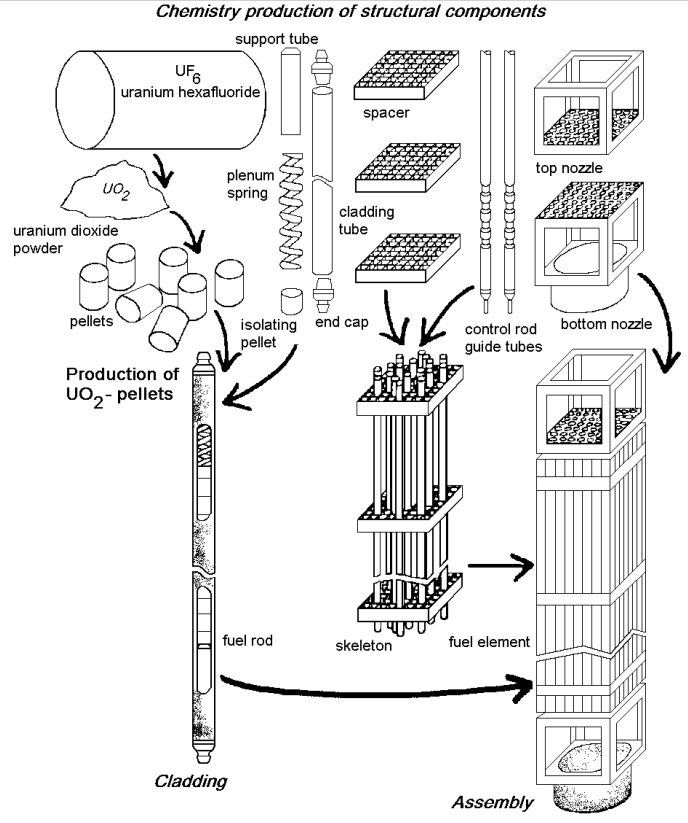
\includegraphics[scale=0.5]{figures/others/nuclear_fuel_rod.png}
    \source{\cite{perrotta1999}.}
    \label{fig:element_structure}
\end{figure}

A operação de reatores nucleares é altamente regulamentada e requer rigoroso controle de segurança, uma vez que acidentes podem resultar em vazamentos de materiais radioativos. A gestão de resíduos nucleares é um desafio crítico, uma vez que os subprodutos da fissão nuclear são radioativos e exigem armazenamento seguro a longo prazo.

\section{Transferência de Calor}

A transferência de calor é a área que estuda como a energia se move entre diferentes corpos ou sistemas. Esse processo ocorre devido à gradientes de temperatura, com a energia sendo transferida do corpo mais quente para o mais frio. O seu estudo possui um papel fundamental no projeto e na otimização de sistemas e dispositivos. O conhecimento do movimento do calor é essencial para garantir a eficiência energética, a segurança e o desempenho adequado em diversas aplicações.

A transferência de calor ocorre por meio de três principais mecanismos: condução, convecção e radiação. A condução é a transferência de energia das partículas mais energéticas de uma substância para partículas vizinhas adjacentes menos energéticas, como resultado da interação entre elas, \citep{cengel2010}. Por outro lado, a convecção é o modo de transferência de energia entre a superfície sólida e a líquida ou gás adjacente, que está em movimento e que envolve os efeitos combinados de condução e de movimento de um fluido, \citep{cengel2010}. Por sua vez, a radiação é a energia emitida pela matéria sob a forma de ondas eletromagnéticas (ou fótons) como resultado das mudanças nas configurações eletrônicas de átomos ou moléculas, \citep{cengel2010}.

À medida que a ciência e a tecnologia avançam, diversos métodos foram desenvolvidos para resolver problemas de transferência de calor, incluindo abordagens analíticas, numéricas (utilizada nesse trabalho e citada anteriormente) e experimentais.

Segundo \citet{maliska2004}, os métodos analíticos e os numéricos formam a classe dos métodos teóricos, pois ambos objetivam resolver equações diferenciais. A diferença está apenas na complexidade da equação que cada método pode atacar. Os métodos analíticos têm a desvantagem de ser aplicáveis apenas em problemas cujas hipóteses simplificativas os desviam demasiadamente do fenômeno físico real. Além disso, são aplicados, normalmente, a geometrias simples e condições de contorno também simples. 

A experimentação numérica (uso de técnicas numéricas), por sua vez, praticamente não apresenta restrições, podendo resolver problemas com complicadas condições de contorno, definidos em geometrias arbitrárias e apresentando resultados com uma rapidez fantástica.

Com relação à experimentação em laboratório, sua grande vantagem é o fato de tratar com a configuração real. Ela é, entretanto, de altíssimo custo e muitas vezes não pode ser realizada, por questões ele segurança, como é o caso da transferência de calor no núcleo de reatores nucleares, ou pela dificuldade de reprodução das condições reais, como, por exemplo, no escoamento supersônico a grandes altitudes ou na simulação de reservatórios de petróleo. Na ausência de modelos matemáticos estabelecidos e em geometrias extremamente complexas, muitas vezes é a única alternativa de que o projetista dispõe.

\subsection{Condução}

A condução de calor visa compreender a transferência de energia das partículas mais energéticas para as menos energéticas decorrente das interações entre partículas em uma material. Para sua descrição, a principal equação utilizada é a Equação da Lei de Fourier, que estabelece que a taxa de transferência de calor (\(q ''\)) é diretamente proporcional à condutividade térmica do material (\(k\)) e ao gradiente de temperatura entre as duas extremidades do material (\( dT / dx \)).

\begin{gather}
    q '' = \dfrac{q}{A} = - k \dfrac{\partial T}{\partial x}
\end{gather}

Essa equação mostra que quanto maior a condutividade térmica do material, maior a taxa de condução de calor. Além disso, a área de seção transversal afeta a taxa de transferência de calor, bem como o gradiente de temperatura. Um gradiente mais íngreme resulta em uma maior taxa de condução de calor.

Segundo \citet{figueiredo2018}, em diversas aplicações, surge o desafio de lidar com variações temporais nas temperaturas, que não se mantêm constantes, como requerido pela Lei de Fourier. Para superar essa dificuldade, faz-se uso da grandeza denominada "fluxo de calor". Através de uma série de considerações e manipulações matemáticas, é possível obter a equação de calor, também conhecida como equação de difusão térmica (apresentada abaixo, na forma retangular).

\begin{gather}
    \dfrac{\partial ^2 T}{\partial x ^2} + \dfrac{\partial ^2 T}{\partial y ^2} + \dfrac{\partial ^2 T}{\partial z ^2} + \dfrac{\dot{q}}{k} = \dfrac{1}{\alpha} \dfrac{\partial T}{\partial t}
\end{gather}

\subsection{Convecção}

A convecção ocorre devido a diferenças de temperatura no fluido, o que leva a variações na densidade e, consequentemente, ao movimento das partículas. A convecção é um mecanismo complexo que envolve a combinação de condução de calor e advecção de matéria. Na convecção, o calor é transferido através do movimento de massas de fluidos quentes em direção a regiões mais frias. Esse movimento é caracterizado por correntes de convecção que podem ocorrer de forma natural, como no caso do aquecimento de ar em uma sala, ou ser pode ser forçado, como em sistemas de aquecimento e ar condicionado.

Apesar da complexidade da convecção, observa-se que a taxa de transferência de calor por convecção é proporcional à diferença de temperatura e está muito bem expressa pela lei de Newton do resfriamento, \citet{cengel2010}.

\begin{gather}
    \dot{q} = h (T_s - T_{\infty})
\end{gather}

Sendo \(h\) o coeficiente de transferência de calor por convecção, \(T_s\) a temperatura da superfície e \(T_{\infty}\) a temperatura do ambiente.

\section{Equações Diferenciais}

Equações diferenciais é uma área fundamental da matemática e da física que descrevem a variação de grandezas em relação a um referencial, em especial o tempo e espaço. Elas são amplamente utilizadas para representar uma variedade de fenômenos, desde o movimento de corpos até o comportamento de sistemas elétricos e dinâmica de fluidos.

Essas equações expressam relações entre uma função e a sua taxa de variação, mostrando como uma variável afeta a outra, e possuindo duas classificações principais: as equações diferenciais ordinárias (EDOs), que envolvem uma única variável independente e as equações diferenciais parciais (EDPs), que lidam com funções de várias variáveis e suas derivadas parciais.

Os métodos para a solução de EDOs e EDPs desempenham um papel crucial na modelagem e resolução de uma ampla gama de problemas em ciência e engenharia. Para EDOs, os métodos analíticos, como a separação de variáveis e o fator integrante, podem ser usados em situações simples. No entanto, para problemas mais complexos e não lineares, os métodos numéricos, como o método de Euler, método de Runge-Kutta e as diferenças finitas, provam ser ferramentas essenciais. Quando se trata de EDPs, os métodos numéricos são amplamente empregados, incluindo os métodos das diferenças finitas, dos elementos finitos e dos volumes finitos. Esses métodos permitem a resolução aproximada das EDOs e EDPs, o que é essencial para abordar problemas complexos que não têm soluções analíticas diretas. Portanto, a escolha do método depende da natureza do problema e da precisão desejada na solução.

\subsection{Método Numérico das Linhas}

Segundo \citet{schiesser2001}, o método numérico das linhas (NUMOL, ou apenas MOL) é uma abordagem abrangente para a solução de problemas de EDP dependentes do tempo que basicamente ocorre em duas etapas: (1) as derivadas espaciais são primeiro aproximadas usando, por exemplo, técnicas de diferenças finitas ou de elementos finitos, e (2) o sistema resultante de EDOs semidiscretas (discretas no espaço - contínuas no tempo) é integrado no tempo. O sucesso deste método decorre da disponibilidade de algoritmos numéricos de alta qualidade e software associado para a solução de sistemas rígidos de EDOs.

A principal ideia por trás do NUMOL é transformar uma EDP em um sistema de EDOs acopladas, substituindo a derivada espacial por diferenças finitas. Isso resulta em um conjunto de EDOs que podem ser resolvidas numericamente por métodos tradicionais, como o método de Runge-Kutta ou o método de Euler, que são amplamente conhecidos e bem estabelecidos. Portanto, o NUMOL divide o domínio espacial em uma série de pontos discretos, formando um sistema de EDOs para cada ponto.

Essa abordagem torna o NUMOL altamente versátil e eficiente, permitindo a simulação de sistemas complexos em que a dimensão espacial é contínua. Além disso, o NUMOL é particularmente adequado para a análise de sistemas transientes, onde as condições podem variar ao longo do tempo. No entanto, como em qualquer método numérico, a escolha de discretização adequada e a precisão da solução dependem da natureza do problema em questão.

\begin{figure}[H]
    \centering
    \caption{Ilustração representativa da origem do método numérico das linhas.}
    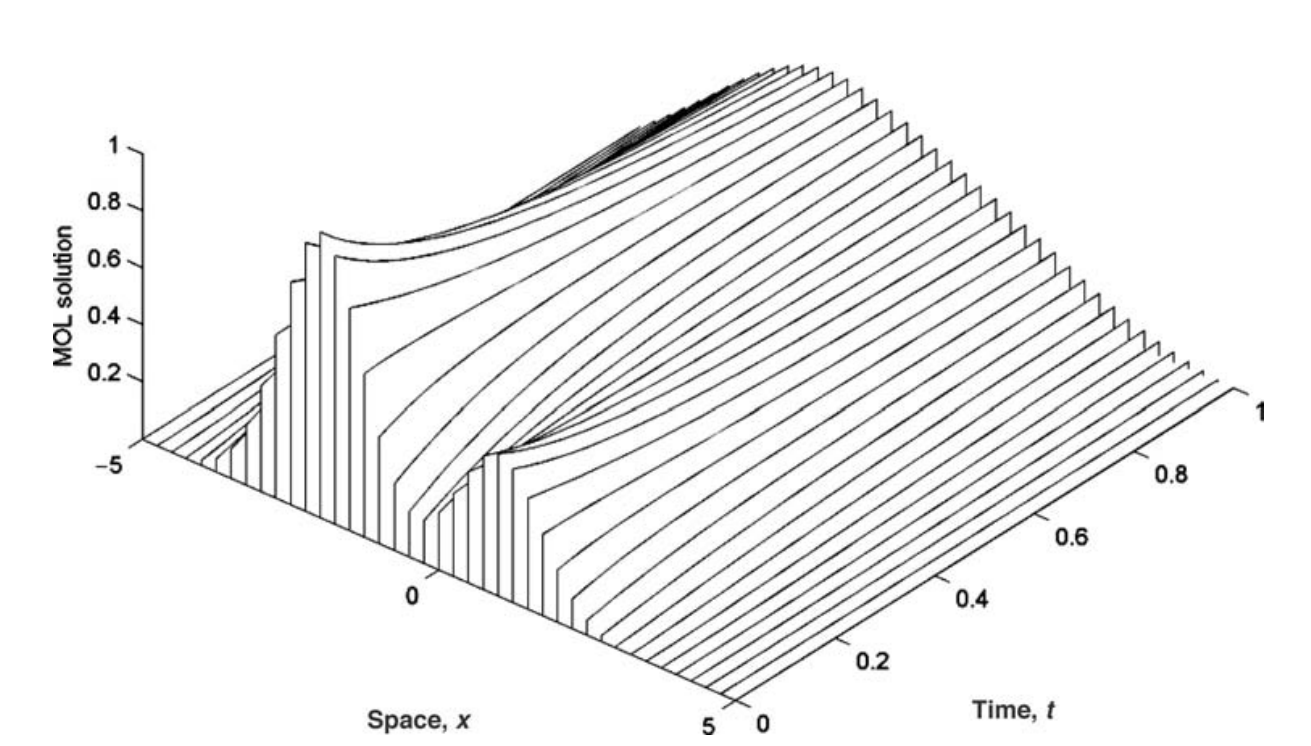
\includegraphics[scale=0.3]{figures/others/method_of_lines.png}
    \source{\cite{schiesser2009}.}
\end{figure}

\subsection{Discretização por Diferenças Finitas}

No contexto do NUMOL, uma variedade de métodos, como as diferenças finitas, elementos finitos e volumes finitos, são empregados para aproximar derivadas espaciais. No caso das diferenças finitas, o domínio de interesse é discretizado em uma grade de pontos, onde essas técnicas são aplicadas em cada ponto.

Essas discretizações variam em ordens de precisão. A primeira ordem utiliza valores em pontos próximos, como nas diferenças progressivas, regressivas e centrais. A segunda ordem, mais precisa, considera valores em pontos adjacentes e usa combinações ponderadas para calcular as derivadas. À medida que a ordem aumenta, a precisão também aumenta, mas a complexidade computacional cresce. Portanto, a escolha da ordem apropriada depende da necessidade de precisão e dos recursos computacionais disponíveis, com ordens superiores sendo preferíveis em cenários que requerem maior acurácia, especialmente em problemas com gradientes intensos ou detalhes finos.

A convergência é um aspecto fundamental para garantir que as soluções numéricas se aproximem das soluções exatas à medida que a discretização é refinada. À medida que reduzimos o tamanho dos intervalos ou aumentamos a quantidade de pontos na grade, esperamos que a solução numérica se aproxime da solução contínua ideal. No entanto, a convergência pode ser afetada por vários fatores, como a escolha do esquema de discretização, as condições de contorno e as características do problema.

Segundo \citep{chapra2008}, a convergência significa que, quando \(\delta x\) e \(\delta t\) tendem a zero, os resultados da técnica por diferenças finitas se aproximam da solução verdadeira. A estabilidade significa que erros em qualquer estágio do cálculo não são amplificados, mas, sim, atenuados conforme os cálculos progridem.

Outro conceito importante é o de estabilidade, que está associado à possibilidade de que pequenos erros introduzidos durante um procedimento matemático possam ser reduzidos à medida que o procedimento continua. Reciprocamente, ocorre instabilidade se pequenos erros tendem a aumentar, talvez sem limite. Se estivermos resolvendo numericamente um problema de valor inicial, o melhor que podemos esperar é que a aproximação numérica tenha comportamento semelhante ao da solução exata. Não podemos transformar um problema instável em um estável simplesmente aproximando sua solução numericamente. No entanto, pode acontecer que um procedimento numérico introduza instabilidade, que não fazia parte do problema original, o que pode causar problemas quando se aproxima a solução. Para evitar tal instabilidade, pode ser necessário colocar restrições sobre o tamanho do passo h, \citep{boyce2020}.
